\chapter{Implementation}
\label{impl}

The following sections contain in-depth descriptions of the design and implementation process of major additions developed throughout this thesis. Less extensive improvements, addressing the security and maintainability of \lcs, are described in appendix \ref{misc}.

\section{Initial State}

At the start of this thesis, a basic version of \lcs had already been implemented. The implementation consisted of the back end server written in \fnurl{Go}{https://golang.org/}, the web interface implemented in \fnurl{AngularJS}{https://angularjs.org/} and the \fnurl{MySQL}{https://www.mysql.com} database. While operational, \lcs was lacking desired functionality. Relevant for this thesis were particularly the weak user registration process, which did not perform any checks to ensure validity of submitted data. When logging in, users were presented with a simple page, merely showing credentials needed to connect to SCIONLab. It was not possible to download configurations and virtual machine images for running SCION. Furthermore, \lcs had no way of communicating with users via email.


This basic implementation was enhanced with new functionality as described in the rest of this chapter.

\section{Email Address Verification}
\label{impl_email_veri}

Two options were evaluated for email verification. Email callback verification and verification based on email exchange.

Email callback verification finds its use mostly as anti-spam measure in \fnote{SMTP}{Simple Mail Transfer Protocol} servers. The verification is carried out in the same way as sending an email to the target email address. However, instead of following through and sending actual email content, the process is aborted as soon as the remote mail exchanger accepts or rejects the recipient address as invalid. The response is the same \code{OK} or \code{Unknown user} as when running the protocol with the intent to send an email. \cite{callback_verification}
Email callback verification, however, suffers from unreliability \cite{callback_verification} which makes it not suitable for \lcs.

Instead, a robust approach based on email exchange was chosen. Upon registration users receive a link with a unique identifier. When they follow the link this is registered by the system and the users' email addresses are marked as verified. Figure \ref{veri:dia} shows a message sequence diagram of the process implemented.

\begin{figure}
	\centering
	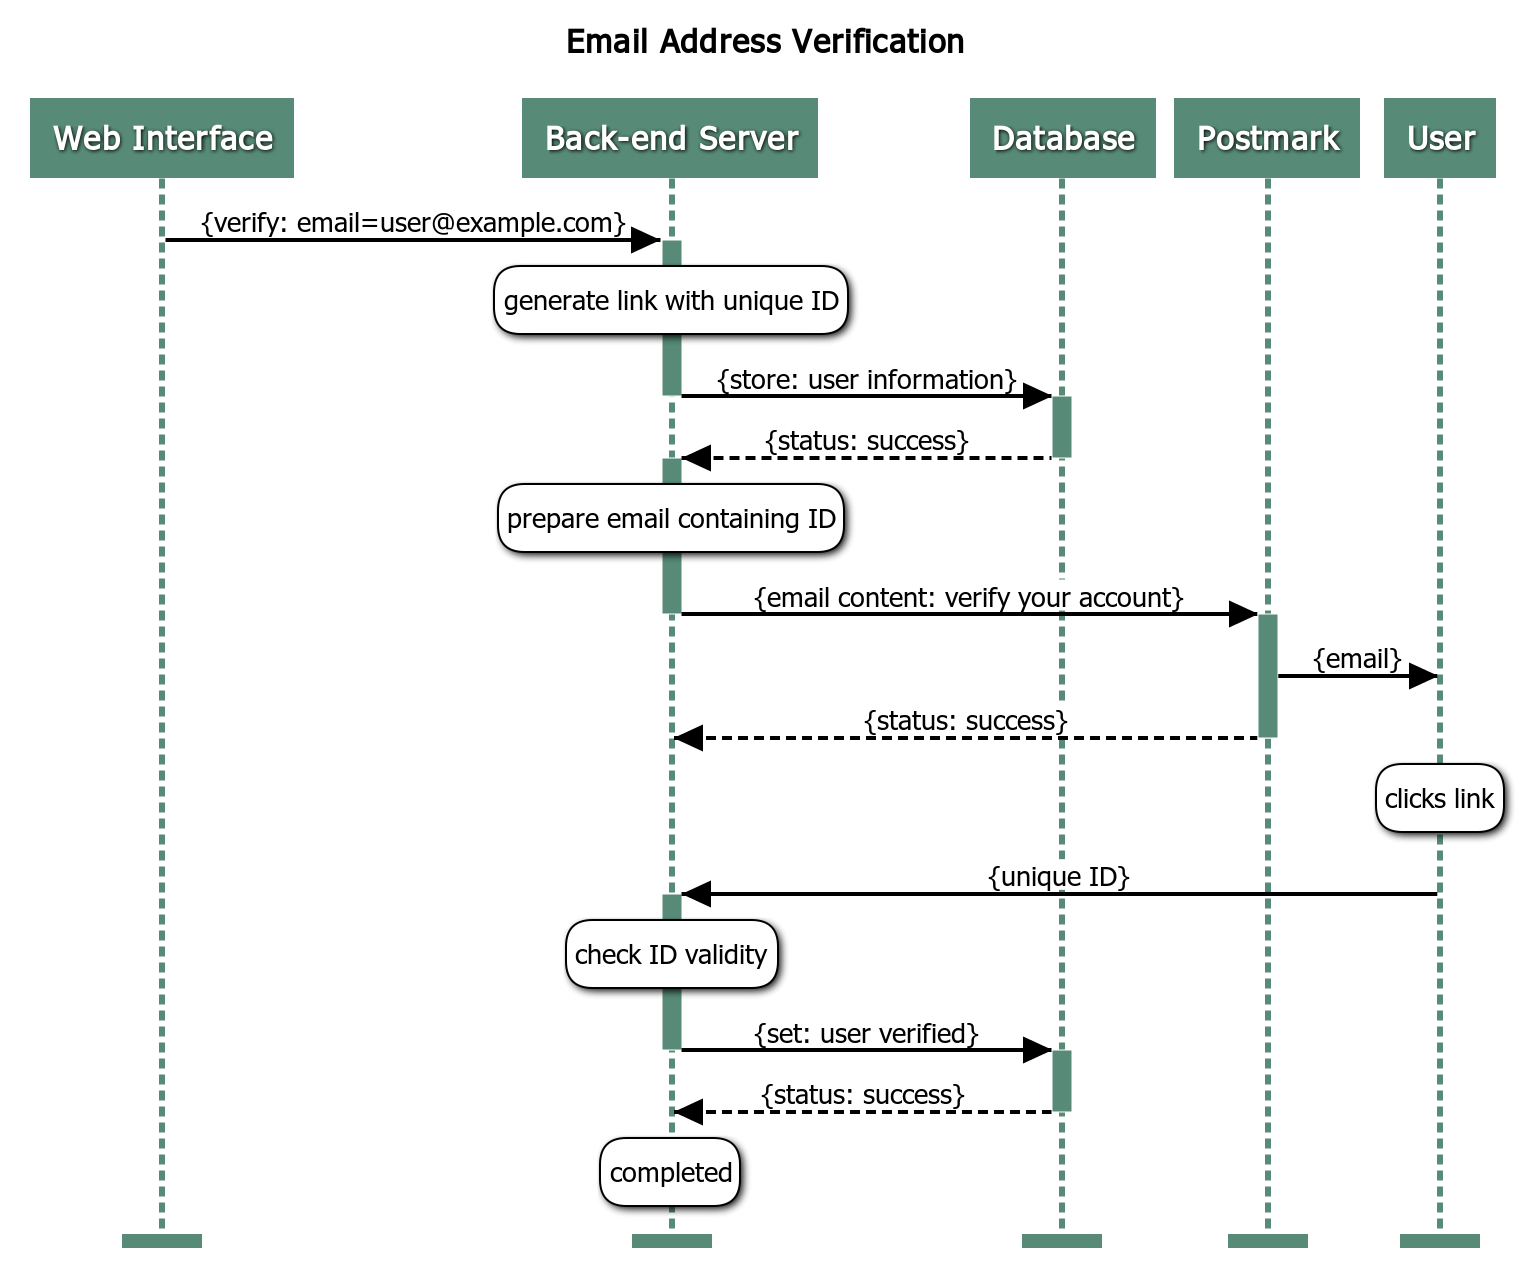
\includegraphics[width=\linewidth]{email_verification.png}
	\captionof{figure}{Sequence diagram showing the messages exchanged for the Email Verification feature}
	\label{veri:dia}
\end{figure}

\subsection{Email package}
\label{impl_email_package}

As already mentioned in Section \ref{archi:postmark}, the initial requirement was to support a local SMTP server for sending emails. Since \lcs originally did not have the ability to send emails, a new, self-written email package was added to the back end server. It was communicating with an \fnote{Exim}{Exim is a popular MTA for UNIX based systems} instance running on the same server. Extensive testing showed that the approach of supporting and maintaining a local MTA is too complex to implement in a reliable fashion for this project. While tweaking the email headers and content was sufficient for the email not to be marked as spam by \fnoteurl{SpamAssassin}{http://spamassassin.apache.org/}{A sophisticated spam filter} (see Figure \ref{exim_spam}), missing \fnote{MX Records}{Mail Exchange Resource Record - A record specifying a mail server in the DNS system} and absent \fnote{DKIM}{DomainKeys Identified Mail - a method to detect email spoofing} authentication (see Figure \ref{exim_auth}) often caused emails to not reach the inbox of users. It was then decided to outsource this complexity to Postmark, as described in Section \ref{archi:postmark}. As a result, the email package was changed to make use of Postmark's APIs, instead of interfacing with the local MTA. The outcome of the same spam detection and authentication tests ran with Postmark as mail provider are shown in Figures \ref{postmark_spam} and \ref{postmark_auth}.

\begin{figure}
	\centering
	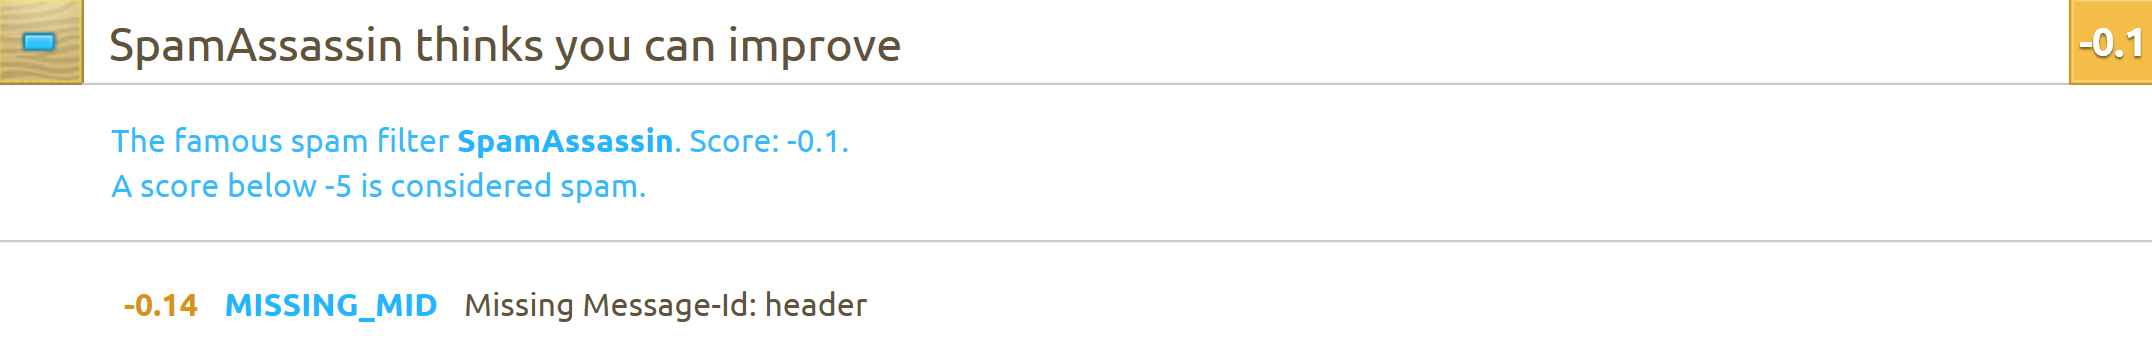
\includegraphics[width=\linewidth]{exim_spamassassin.png}
	\captionof{figure}{Result of SpamAssassin ran against local Exim SMTP server (Run on \href{https://www.mail-tester.com/}{Mail-Tester})}
	\label{exim_spam}
\end{figure}

\begin{figure}
	\centering
	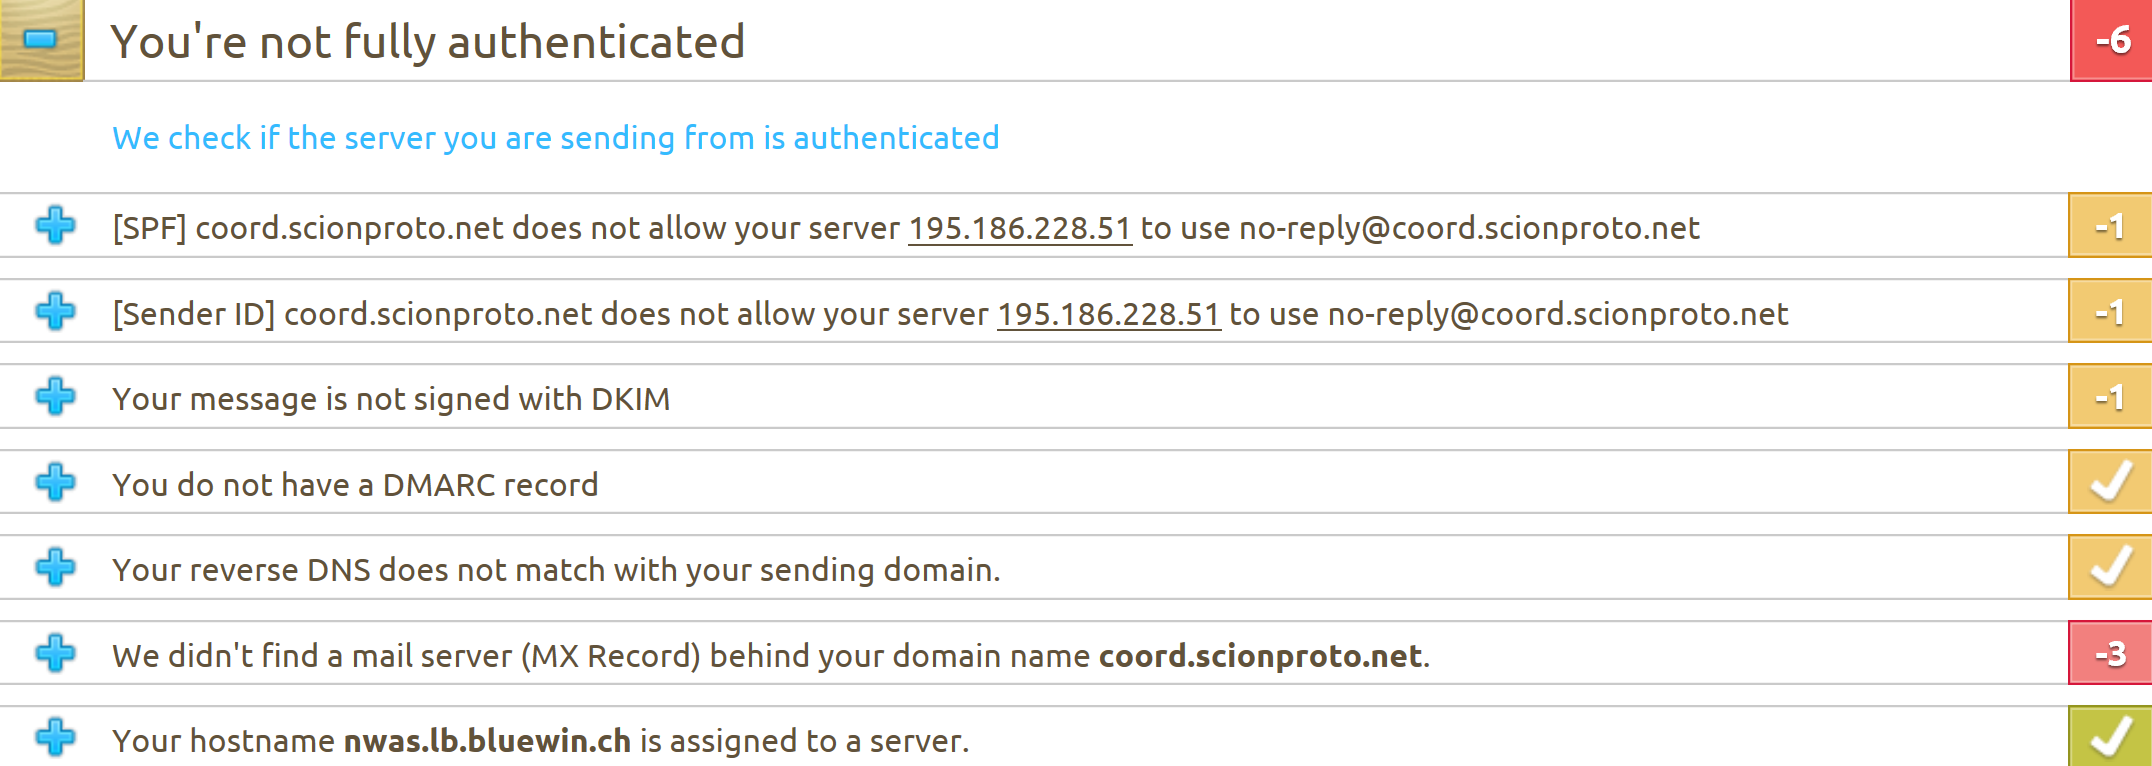
\includegraphics[width=\linewidth]{exim_auth.png}
	\captionof{figure}{Authentication report for the local Exim SMTP server (Run on \href{https://www.mail-tester.com/}{Mail-Tester})}
	\label{exim_auth}
\end{figure}

\begin{figure}
	\centering
	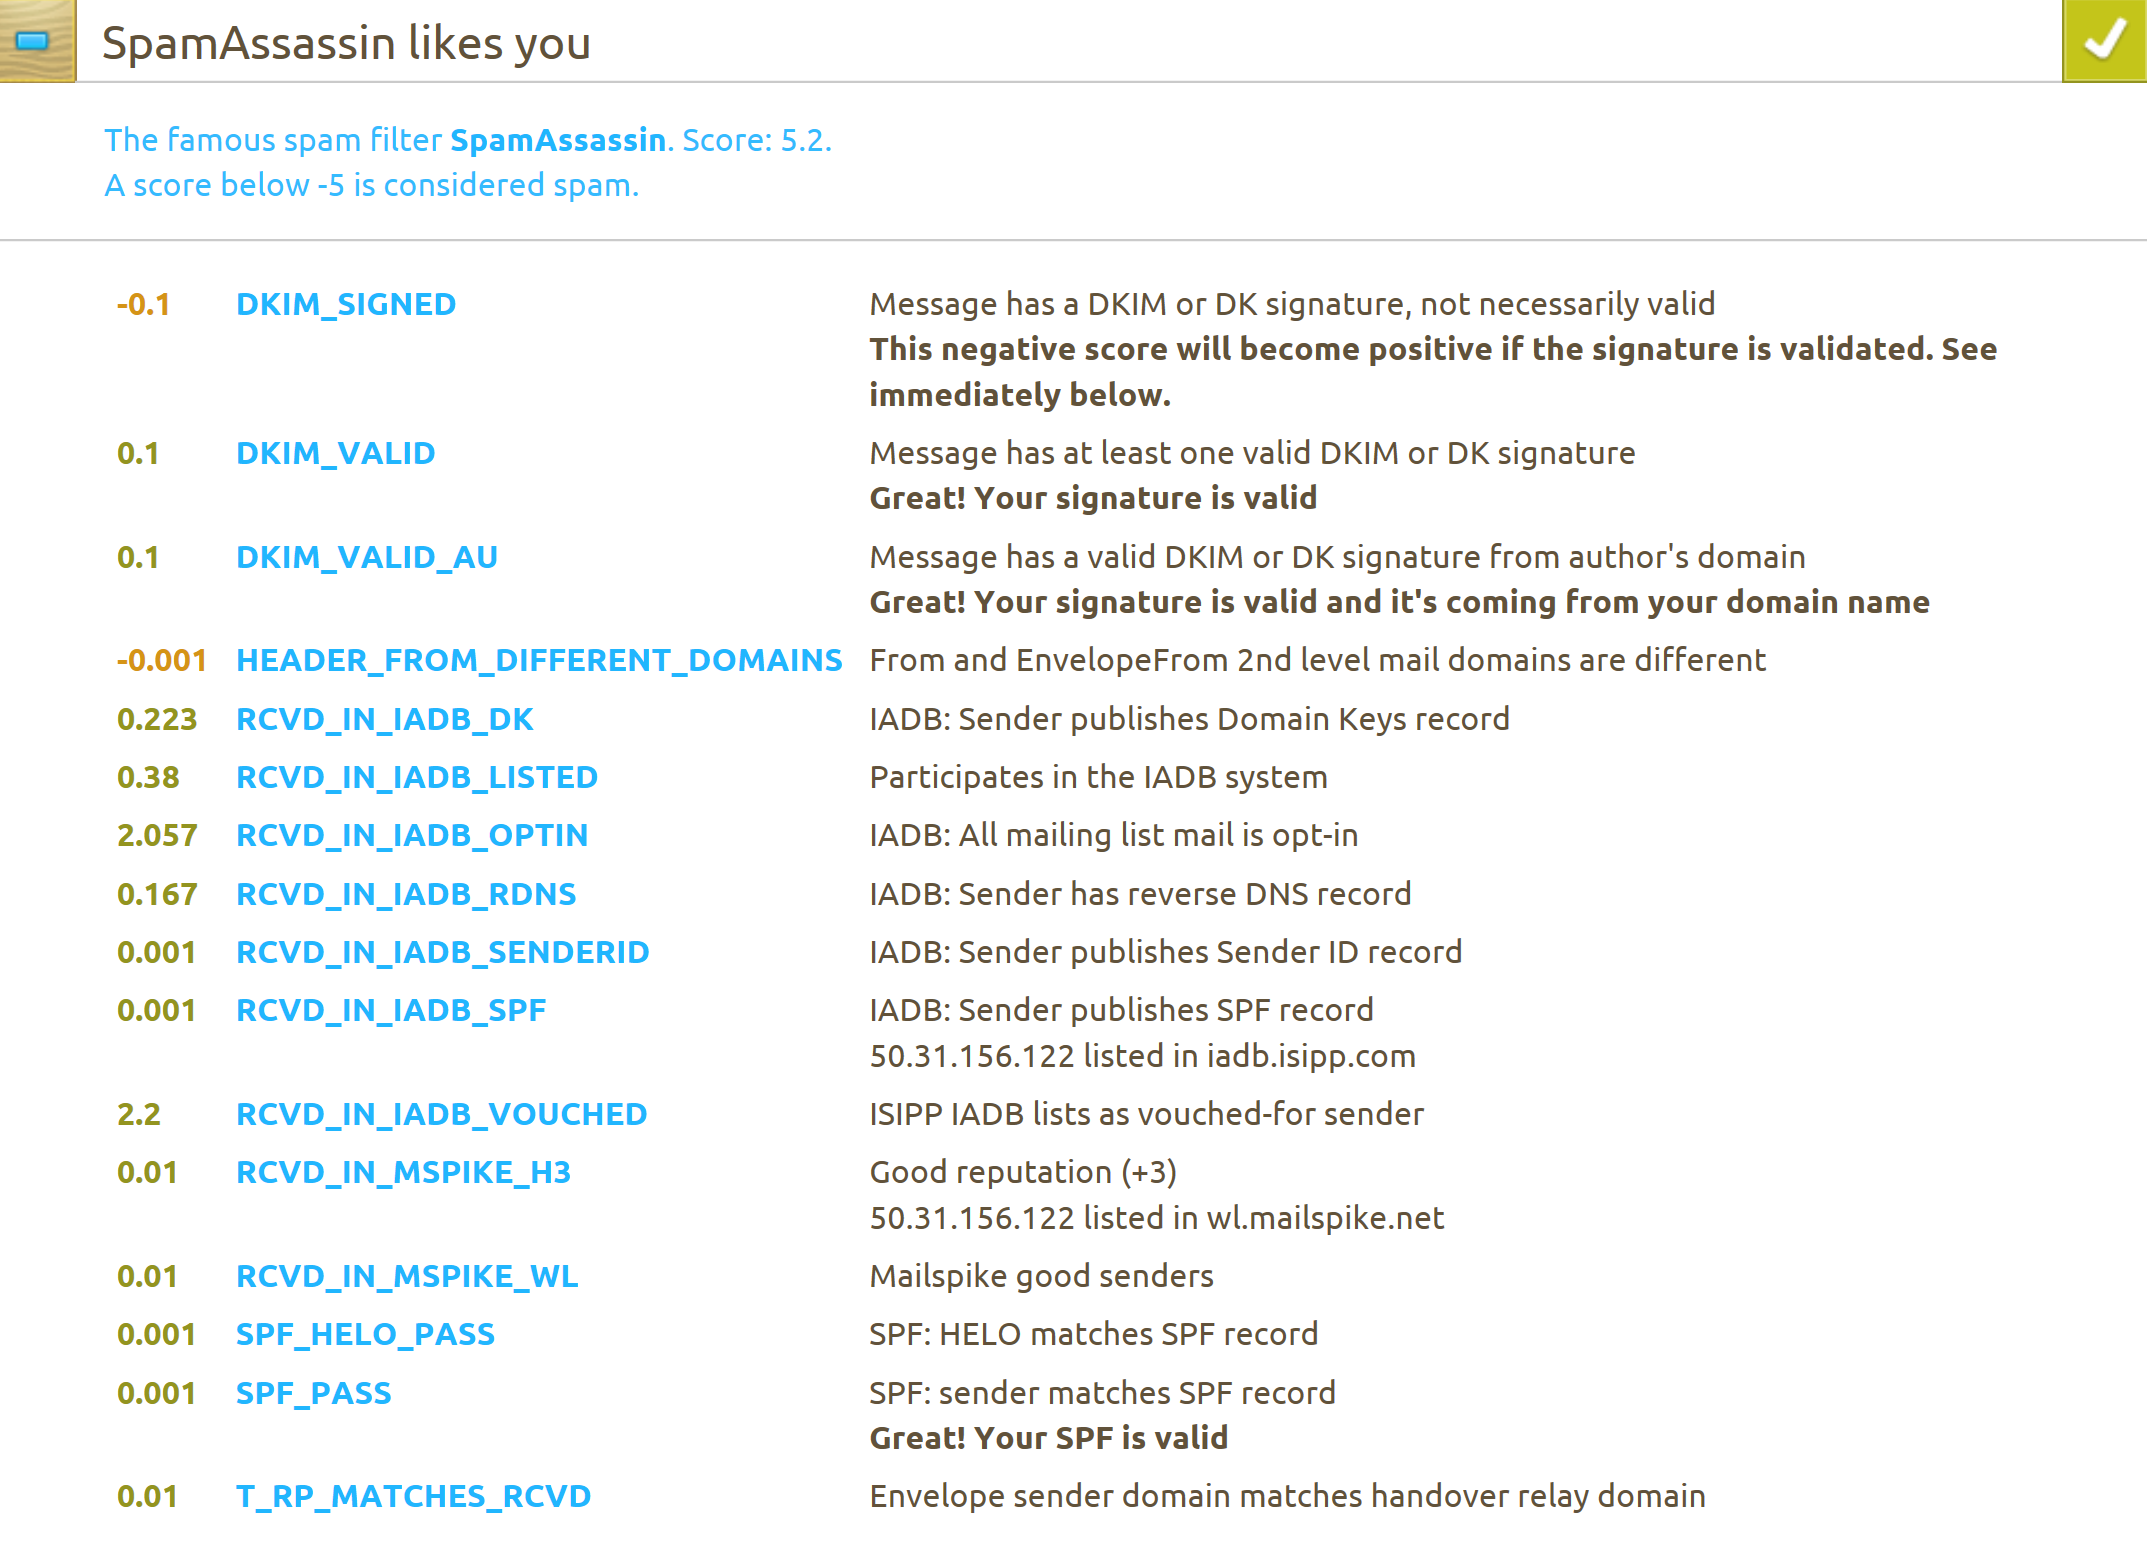
\includegraphics[width=\linewidth]{postmark_spamassassin.png}
	\captionof{figure}{Result of SpamAssassin ran against Postmark (Run on \href{https://www.mail-tester.com/}{Mail-Tester})}
	\label{postmark_spam}
\end{figure}

\begin{figure}
	\centering
	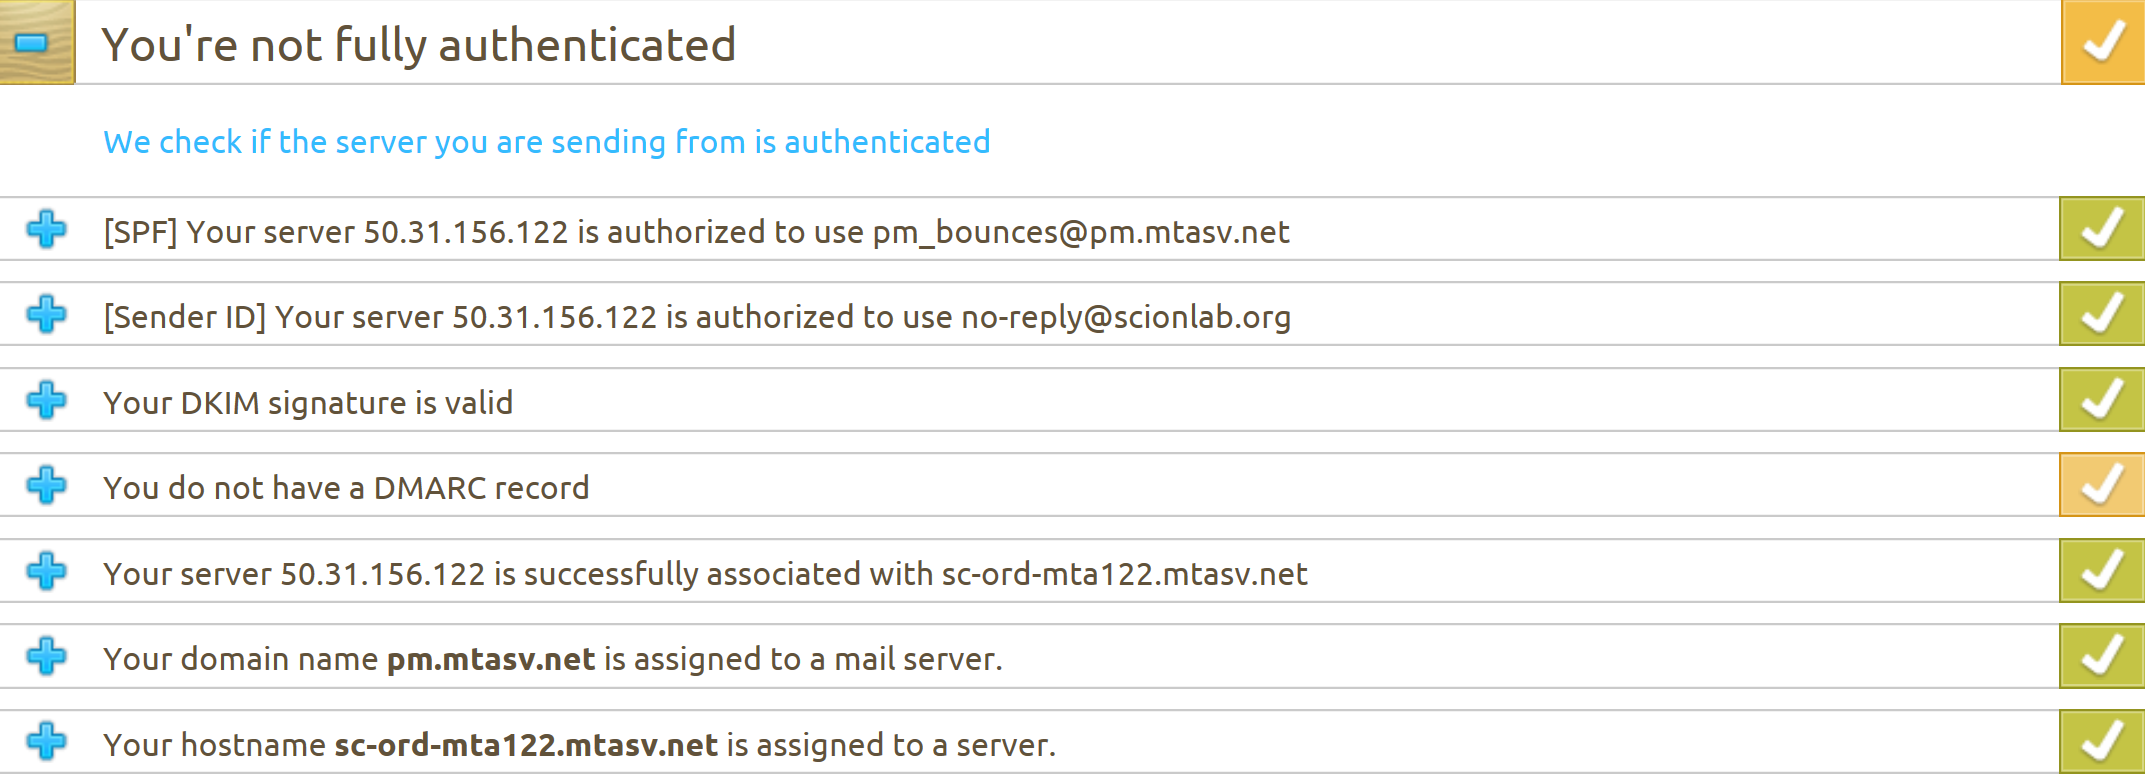
\includegraphics[width=\linewidth]{postmark_auth.png}
	\captionof{figure}{Authentication report for Postmark (Run on \href{https://www.mail-tester.com/}{Mail-Tester})}
	\label{postmark_auth}
\end{figure}

\subsection{Adapted Components}

Apart from the added email package, other components had to be adapted to implement the feature. The following functionality was added:

\subsubsection{User information on Web Interface}
On the web interface, an alert box was integrated on the registration page. Upon successful registration it asks the user to check his emails. Otherwise it displays an error corresponding to the problem that occurred.

\subsubsection{Email creation}
The existing code to register a new user was extended to additionally prepare a personalized email, containing the verification link. This email then gets sent using the email package. The unique identifier contained in the link is stored in the database together with the user information. This allows for a direct mapping between user and identifier.

\subsubsection{Verification API}
A new API was added for handling email address verification requests. This API gets called by the user's web browser when following the confirmation link. Listing \ref{lst_verify_api} shows the signature of the API. \code{uuid} denotes the per-user unique identifier.

\begin{lstlisting}[language=golang, caption={API signature for verifying an email address}\label{lst_verify_api}, float]
//email validation
router.Handle("/api/verifyEmail/{uuid}",loggingChain.ThenFunc(
	registrationController.VerifyEmail))
\end{lstlisting}
%floatplacement=whatever as argument possible

\subsubsection{Handler Function}
A new handler function which gets invoked by the above API call. It checks that the identifier sent in the request is valid and belongs to a user with a not yet verified email address. If the identifier is valid, the corresponding user is set to verified and a confirmation page gets served to the web browser. If not, an error is logged and forwarded to the web browser.

\subsubsection{Confirmation Page}
A confirmation page informing the user about the successful verification process was added to the web interface. This is the page served by the handler function on successful verification. It offers a shortcut to the login page.

\section{Manual User Activation}
\label{impl_user_activation}
The manual user activation feature builds on top of the email verification system. After verifying the email address a user should not immediately be granted access to \lcs. A second verification step is required. The user needs to be activated. To make the process of user activation as automated as possible we distinguish between two cases. Either the user's email address is on a list of pre-defined, trusted domain names. In this case the activation is done automatically. In case the email's domain name is not on the list, the user has to be manually approved by an administrator. Manual activation happens through a newly designed administrator panel added to the web interface. The process with it's two cases is outlined in Figure \ref{acti:dia}. The notification emails sent to administrators and users make use of the new email package introduced for the email verification system.

\begin{figure}
	\centering
	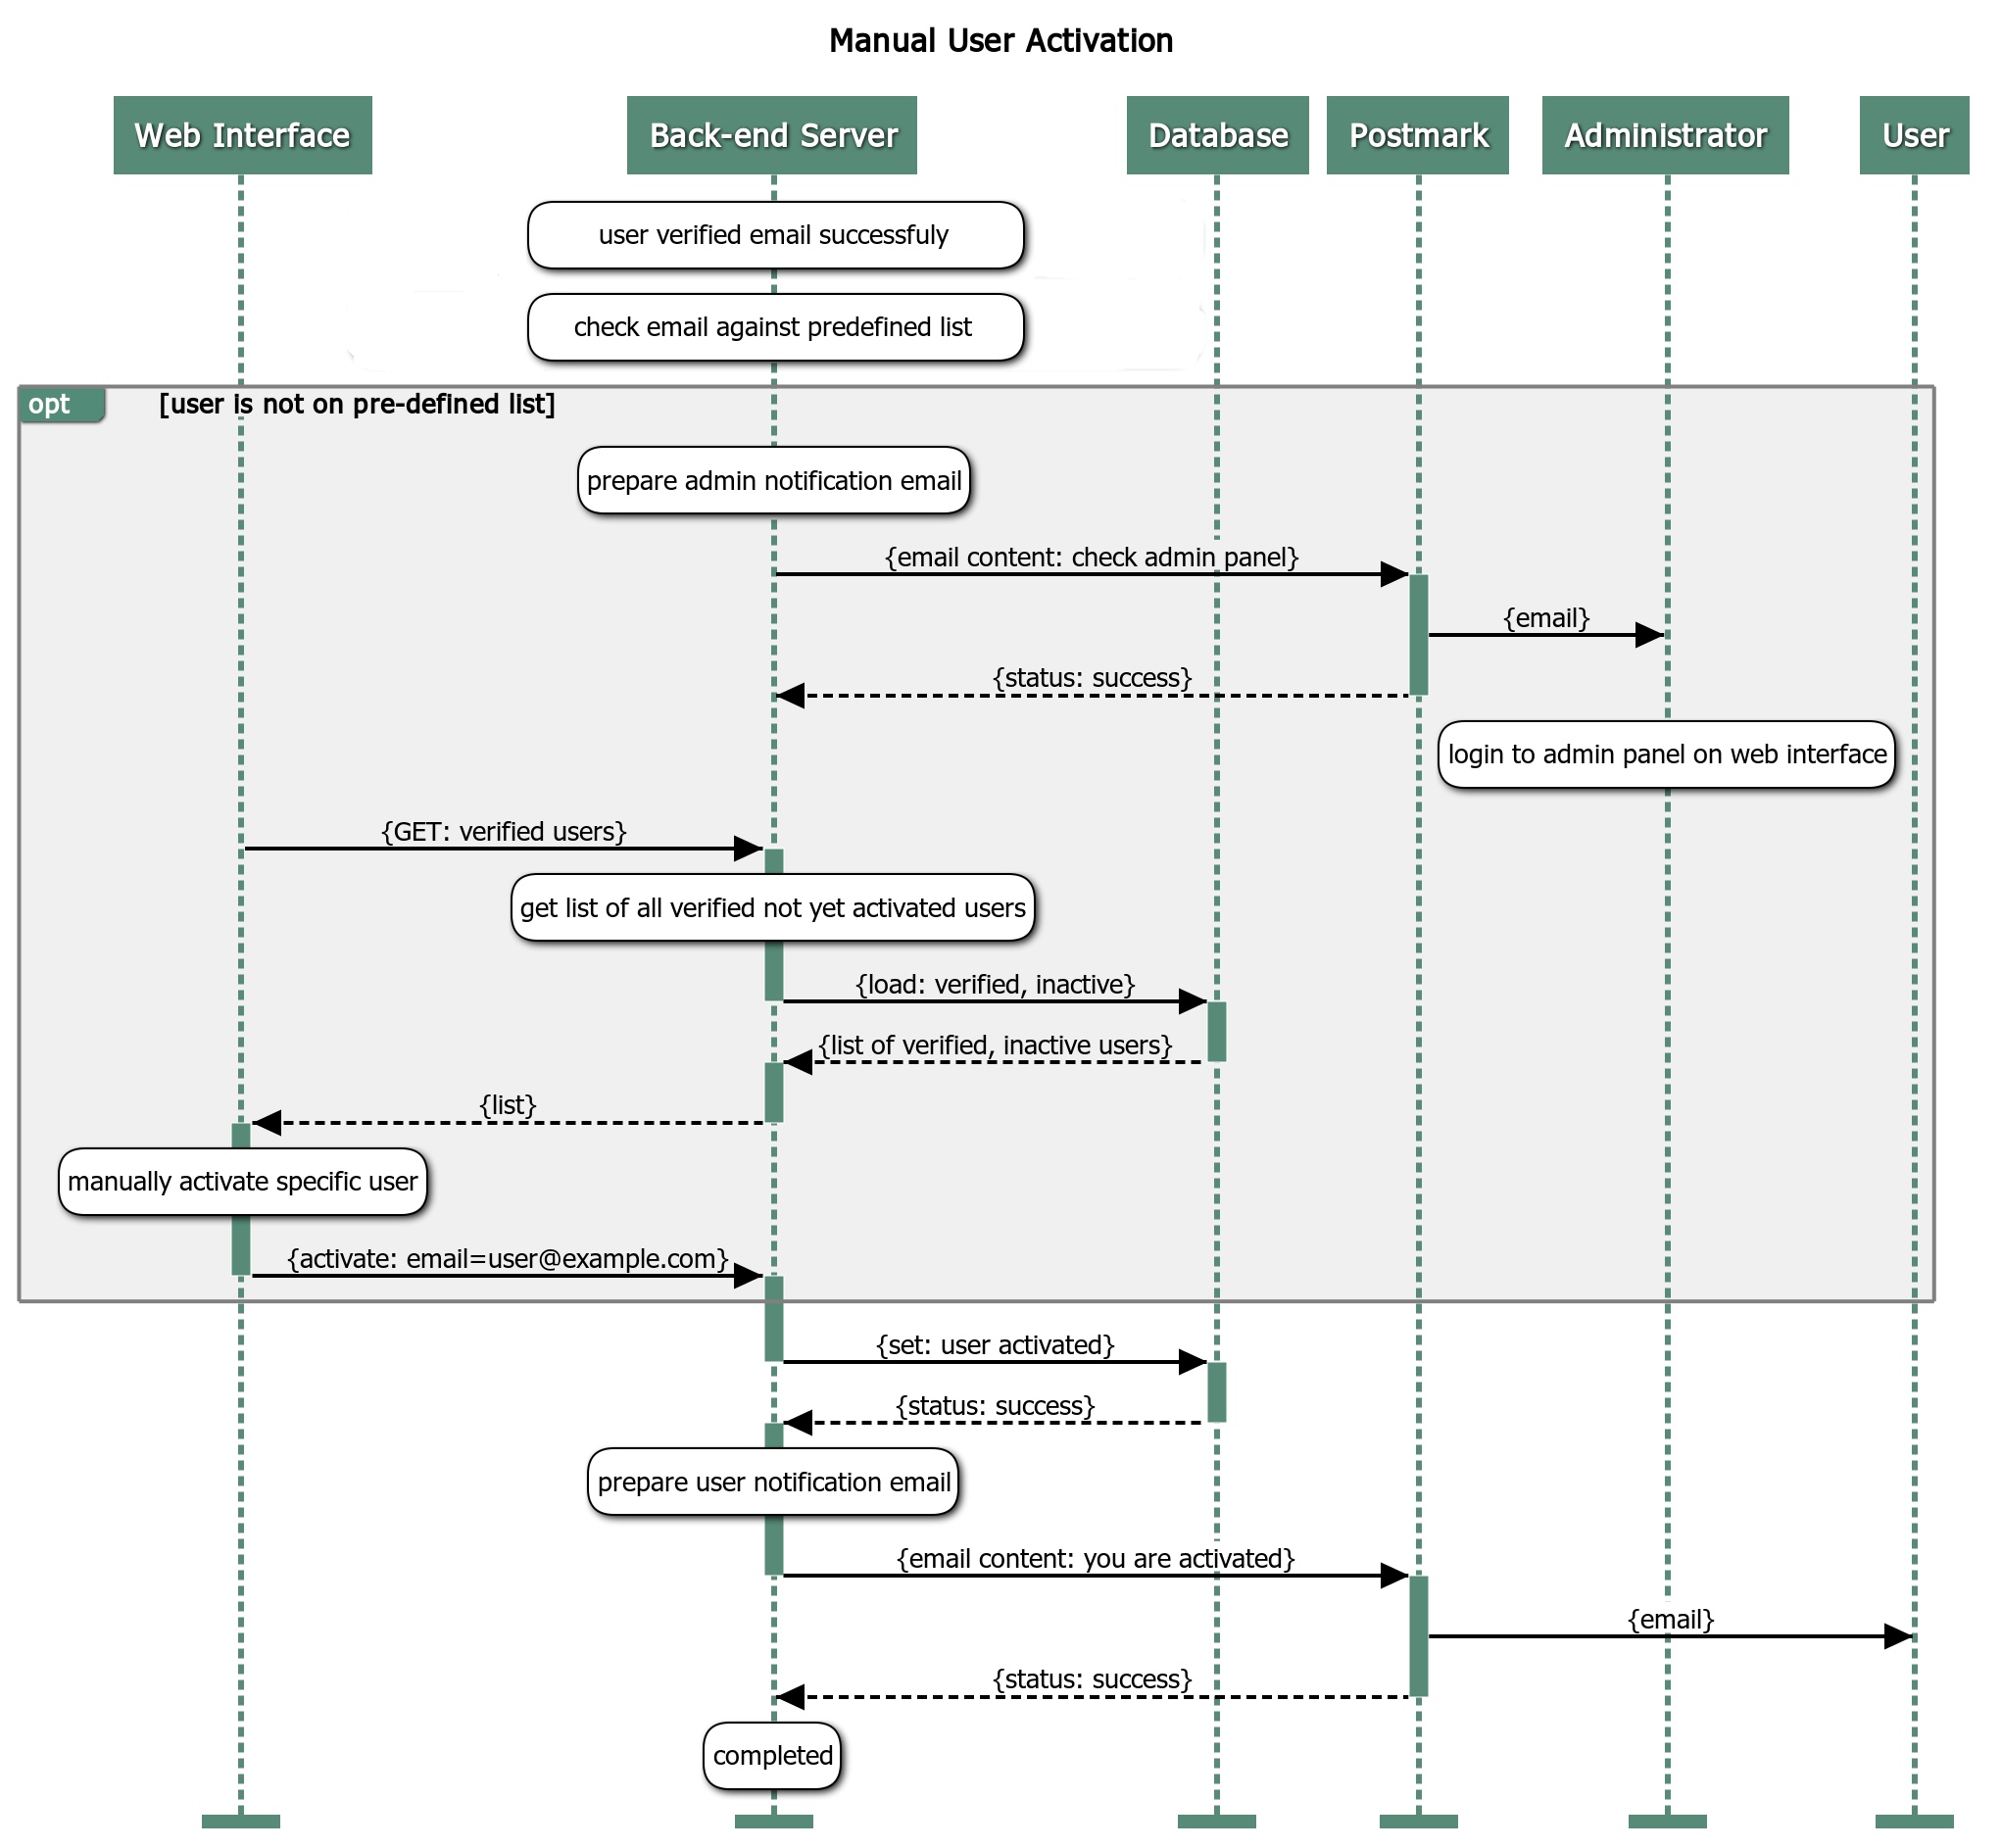
\includegraphics[width=\linewidth]{manual_user_activation.png}
	\captionof{figure}{Sequence diagram showing the messages exchanged for the Manual User Activation feature}
	\label{acti:dia}
\end{figure}

\subsection{Role based access control}
In order to activate a regular user by an administrator the concept of different user groups had to be introduced to \lcs. For this purpose the system was adapted to support a simple role based access control model (RBAC). Instead of granting special rights to individual users each user gets instantiated with a role that reflects the rights this user should possess. This model easily supports many different roles with distinct sets of permissions. However, for the user activation feature only two roles were needed; an administrator role and a regular user role. The regular user role is the role assigned to standard users when signing up through the web interface of \lcs. The administrator role possesses all the permissions of the regular user role and additionally the ability to log in to the administrator panel via the web interface, from where regular users can be activated.

\subsection{Adapted Components}

On top of the changes made to implement the RBAC model the following enhancements were made to support the user activation feature:

\subsubsection{Admin User Creation}
We mentioned above that creating a user through the web interface assigns the regular user role. In order to bootstrap administrator creation, \lcs was extended to accept command line arguments that allow the creation of administrators on system start up. Administrators could then be used to create other administrators. However, such functionality is not in place yet.

\subsubsection{Activation API}
Activating users through the administrator panel requires the web interface to issue two types of requests to the back end server (see Figure \ref{acti:dia}). First, it retrieves a list of all verified, not yet activated users. Then, for a selected user, it issues an activation command. The signature of these two API calls are shown in Listing \ref{lst_acti_api}.

\begin{lstlisting}[language=golang, caption={API signatures for loading unactivated users and for activating users}\label{lst_acti_api}, float]
// user activation
router.Handle("/api/loadUnactivatedUsers", loggingChain.ThenFunc(
	loginController.LoadUnactivatedUsers))
router.Handle("/api/activateUser", loggingChain.ThenFunc(
	loginController.ActivateUser)).Methods("POST")
\end{lstlisting}

\subsubsection{Handler Functions}
Corresponding to the APIs in Listing \ref{lst_acti_api}, \lcs was extended with two new handler functions. \code{LoadUnactivatedUsers} first checks if the request was issued by an administrator. If this is the case it retrieves a list of all verified, inactive users from the database and sends it back in the HTTP response. Otherwise an error is sent to the web interface.

The second handler function, \code{ActivateUser}, performs the same administrator authentication check and, on success, activates the user corresponding to the email address contained in the request. If the authentication fails, the handler responds with an error.

\subsubsection{Email Notifications}
Using the email package introduced in Section \ref{impl_email_package}, new notification emails were added to \lcs:

An email gets sent to all administrators when there are new users waiting to be activated in the administrator panel. This ensures that users who can not be activated automatically are not waiting too long for their activation. This email is sent once there are pending users, rather than for every individual user.

When a user gets manually activated, an email informing about the changed status gets sent to that user. It contains a link to the login page of the web interface.

\subsubsection{Pre-defined List}
In Section \ref{impl_user_activation} we mentioned that users with a trusted email address get activated automatically after they verify their email address. In order to implement this feature, trusted email domain names are collected in a list that comes as part of the \lcs configuration.

The following formats are possible:

\begin{itemize}
	\item example@domain.tld (full email address)
	\item domain.tld (domain \& \fnote{TLD}{Top Level Domain})
	\item sub1...sub2.domain.tld (subdomains \& TLD)
	\item tld (TLD only)
\end{itemize}

Upon successful verification, it is checked whether or not the email is on the list. If the address matches an entry, it is immediately activated. Otherwise the user must go through the manual activation process.


\subsubsection{Administrator Panel}
A new administrator panel was added to the web interface. It displays a table containing all verified, inactive users together with their relevant information like name, email address and organisation. Individual users can be activated via an activation button.

\subsubsection{Confirmation Page}
The confirmation page displayed when users follow the email verification link was revamped to provide users who can not be activated automatically with information about the extended activation process.

\section{CAPTCHA Integration}
\label{impl_capt}

Fake accounts can negatively impact the performance of a system, and with email sending involved in the registration process, bots can abuse \lcs for spamming. As counter measurement against such malicious behaviour, a CAPTCHA was placed on the registration page. The interaction of users with the CAPTCHA and its overall integration into \lcs can be seen in Figure \ref{capt:dia}.
  
\begin{figure}
	\centering
	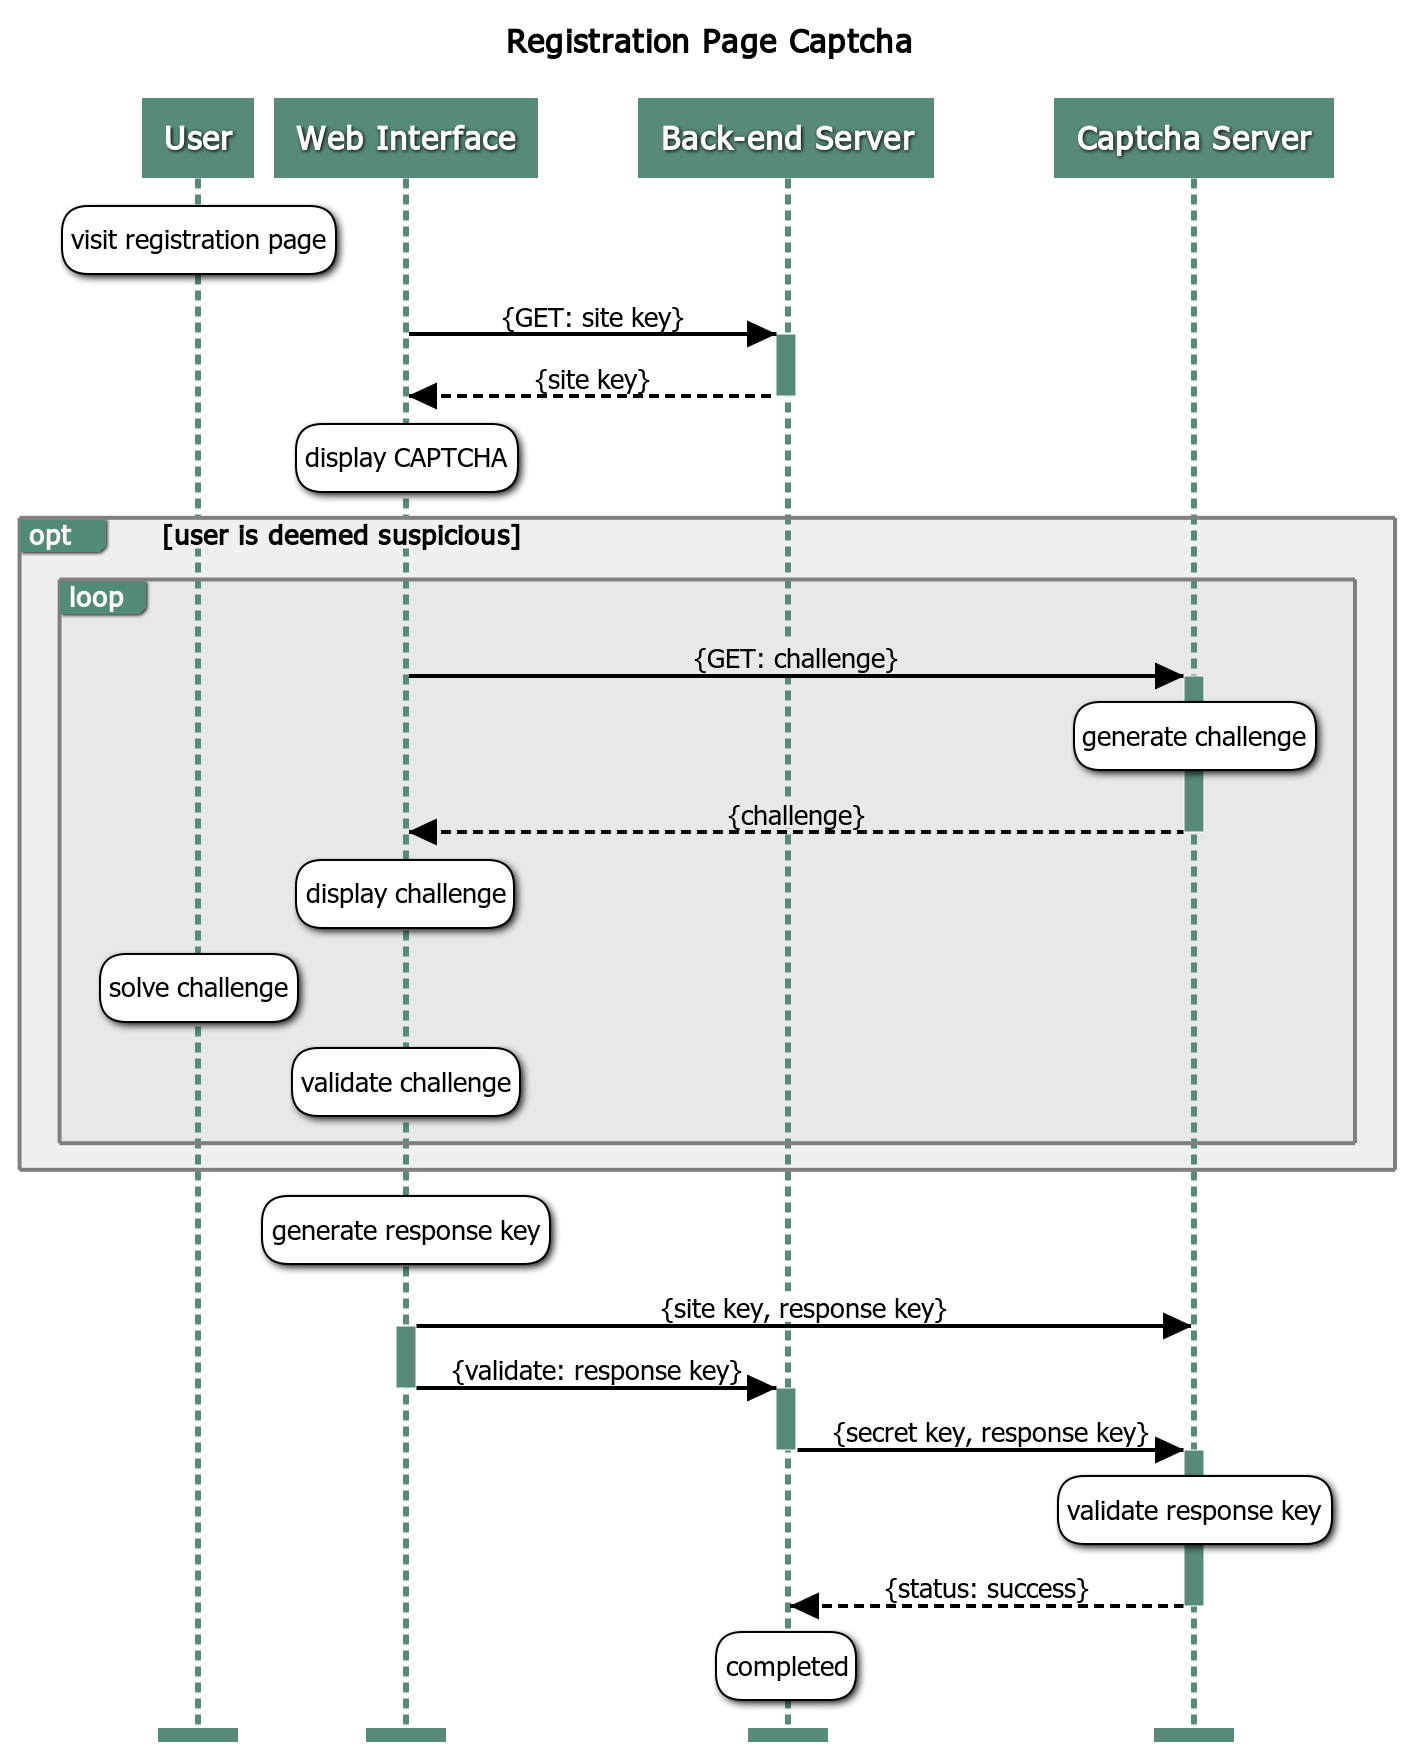
\includegraphics[width=\linewidth]{captcha.png}
	\captionof{figure}{Sequence diagram showing the exchanged messages for the CAPTCHA implementation}
	\label{capt:dia}
\end{figure}


\subsection{Google reCAPTCHA}
For \lcs, Google \fnurl{reCAPTCHA}{https://www.google.com/recaptcha/intro/android.html} was chosen as CAPTCHA provider for a variety of reasons: Since reCAPTCHA is the most popular CAPTCHA service many users will be familiar with how it works. \cite{google_recaptcha} Also, thanks to its advanced risk analysis which observes a user's interaction with the website to infer whether a user is human, often users are not forced to solve a challenge to pass the Turing test. A mere click on a check box is enough to pass.  \cite{google_recaptcha} This effortless verification for human users complies with the non-functional requirements of \lcs outlined in Section \ref{non-func_req}. 
Furthermore, reCAPTCHA is very well supported and documented by Google which makes implementation straight forward.

reCAPTCHA uses a set of keys to fulfill its task. The web page containing the reCAPTCHA must be registered to obtain a site key and a secret key. The site key is used to create reCAPTCHA response keys for users passing the Turing test. This response key then gets verified by sending it to a reCAPTCHA server together with the secret key. Additionally, the reCAPTCHA server provides the reCAPTCHA widget on the web page with challenges to be solved. 

\subsection{Adapted Components}

In order to implement the reCAPTCHA for the registration page of the web interface the following changes had to be made to the system:

\subsubsection{CAPTCHA API}

On the web interface reCAPTCHA must be instantiated with the site key corresponding to the web page it is placed on. When the page loads this site key is retrieved via an API call from the back end server. This offers the convenience of having all keys stored in the main configuration file of \lcs rather than hard coding the site key into the web page. Like this, if new keys need to be installed or \lcs is deployed onto another machine, only the configuration file has to be changed. 

The response key gets appended to the user information as an attribute and is sent using the existing registration API call to the back end server where it is validated together with other user information.

The described endpoints are shown in Listing \ref{lst_captcha_api}

\begin{lstlisting}[language=golang, caption={API signatures for registering users and loading the captcha site key}\label{lst_captcha_api}, float]
// user registration
router.Handle("/api/captchaSiteKey", loggingChain.ThenFunc(
	registrationController.LoadCaptchaSiteKey))
router.Handle("/api/register", loggingChain.ThenFunc(
	registrationController.Register)).Methods("POST")
\end{lstlisting}

\subsubsection{Handler Functions}

The newly added \code{LoadCaptchaSiteKey} handler retrieves the site key from the configuration and hands it over to the web interface where it is used to instantiate the reCAPTCHA.

When a user submits his registration information, the existing \code{Register} handler is triggered. It reads the user data, including the response key, from the request and performs validity checks on the submitted information. The following new check was added to this phase:
The site key is sent together with the secret key to the reCAPTCHA sever, which in turn verifies whether or not the response key is valid for the site specified by the secret key. Here, communication with the reCAPTCHA server is done using the third party \fnurl{haisum/recaptcha}{https://github.com/haisum/recaptcha} package. If all checks pass, the user's information is stored in the database.

\subsubsection{CAPTCHA Widget on Registration Page}

Using the \fnurl{VividCortex/angular-recaptcha}{https://github.com/VividCortex/angular-recaptcha} AngularJS directive, the reCAPTCHA widget was placed on the registration page. Solving the reCAPTCHA was made mandatory for sending registration data to the back end.

\section{CircleCI Integration}
\label{impl_ci}

In Section \ref{archi:ci} we talked about CircleCI and how it helps with the software verification process. Every time a pull request is updated with new code CircleCI runs a defined suite of tests in the cloud. For this to work CircleCI must know about the project environment, what dependencies are used and what tests it has to run. This information is pulled from a configuration file that resides in a special folder inside the \lcs code base. These configurations are processed and used to create a minimal, virtual environment in the CircleCI cloud, which is able to run the code to be tested. The contents of the configuration file is shown in Listing \ref{lst_ci}.

The following subsections describe how CircleCI is set up in order to run the test suite. 

\lstinputlisting[language=yaml,caption={CircleCI project configurations}\label{lst_ci}, float]{code/ci.yml}

\subsection{Environment}
The easiest way to set up the required environment is to use a pre-defined \fnoteurl{Docker}{https://www.docker.com/}{Docker bundles software in isolated containers, then runs these containers on a host system using virtualization} image that comes bundled with all the tools needed for the testing and debugging process.

As can be seen on line 6 and 12 in Listing \ref{lst_ci}, two Docker images are used:
The \code{circleci/golang:1.8} image is an image built by CircleCI specifically for testing Go code. It comes with the Go 1.8 environment and numerous other useful tools, such as Git and SSH, pre-installed.

\code{circleci/mysql:latest} additionally installs the latest version of MySQL in the test environment, which is crucial since tests involve storing to and loading from the database. This image also allows setting up the database in a way such that it conforms to what \lcs is expecting. (see lines 8 to 10 of Listing \ref{lst_ci})

\subsection{Dependencies}
\lcs uses many dependencies which all need to be installed for tests to run successfully. Dependencies are downloaded using the Go command \code{go get -v -t -d ./...}. This downloads all needed packages and writes the name of each package to the test log.

\subsection{Testing}
\code{go test -v ./...} looks for all test files in the code base and then runs the test cases one by one. For each test case it writes status information to the log file stating whether the test failed or not. In case of failure, a corresponding error message is logged as well.

\section{Deployment with Ansible}
\label{impl:ansi}

In Section \ref{archi:ansi} we described how Ansible supports the deployment process. As with CircleCI, Ansible needs instructions to put the target machine into the right state and to deploy \lcs correctly. The most important configurations are described below.


\lstinputlisting[language=yaml, linerange={1-20}, caption={Excerpt of Ansible tasks, used to set up \lcs}\label{lst_ansi_tasks}, float]{code/ansi_tasks.yml}

\begin{lstlisting}[language=yaml, caption={Excerpt of the Ansible parameter file used for \lcs}\label{lst_ansi_param}, float]
mysql_db: scion_coord_test
mysql_pass: development_pass
\end{lstlisting}


\subsection{Hosts}
The host configuration file contains sections for different roles to deploy. Within each section, the addresses of the machines assigned to this role are specified; therefore creating a one-to-many relation between roles and machines.

In the case of \lcs there is only one role, as the complete architecture runs on a single machine.
However, by specifying multiple addresses, the service could easily be replicated for redundancy.

\subsection{Files}
Ansible is capable of copying entire files to a target machine. In \lcs this is used to apply SSH keys and a \fnote{sudoers file}{A file containing rules that users must obey when the sudo command is used} to the deployment environment. This sets up the environment with the necessary user account permissions, required to run \lcs.

\subsection{Parameters}
Certain parameters used in tasks are confidential, do change frequently or are not the same for every target machine. To avoid duplication of playbooks, Ansible allows the use of place holders in tasks.

For simplicity, place holders used in \lcs are compiled in a dedicated parameter file, together with their corresponding values. Lines 13 and 15 of Listing \ref{lst_ansi_tasks} show how place holders are used in a task to confidentially set the password for the MySQL root user. Listing \ref{lst_ansi_param} shows the corresponding excerpt of the parameter file.

\subsection{Tasks}
Ansible runs for each target machine a set of tasks (a playbook), dependant on the assigned role. If tasks are written carefully, the process of running them is idempotent, which means that running the tasks multiple times has no further effect. Idempotence is one of the core concepts of Ansible. It allows tasks to be written in a descriptive way, such that they only get executed when the current state of the machine violates the desired end state. This speeds up the deployment process and prevents data loss caused by writing files which already exist. After completing all tasks, the target machine is in a state that conforms to the state described by the playbook.

Tasks for deploying \lcs consist of installing required packages, setting up the database, applying SSH keys and checking out the code base. Listing \ref{lst_ansi_tasks} shows an excerpt of the playbook used to deploy \lcs. Lines 2-8 show how required packages are installed. As described above, if a package already exists it will not be downloaded again. This speeds up the deployment. Similarly, tasks for setting up the database (lines 10-20) only run when needed to reach the end state, preventing data loss in case the database already exists.